% \documentclass[border=10pt]{standalone}
% \usepackage{tikz}
% % \usepackage{stmaryrd}

% \begin{document}

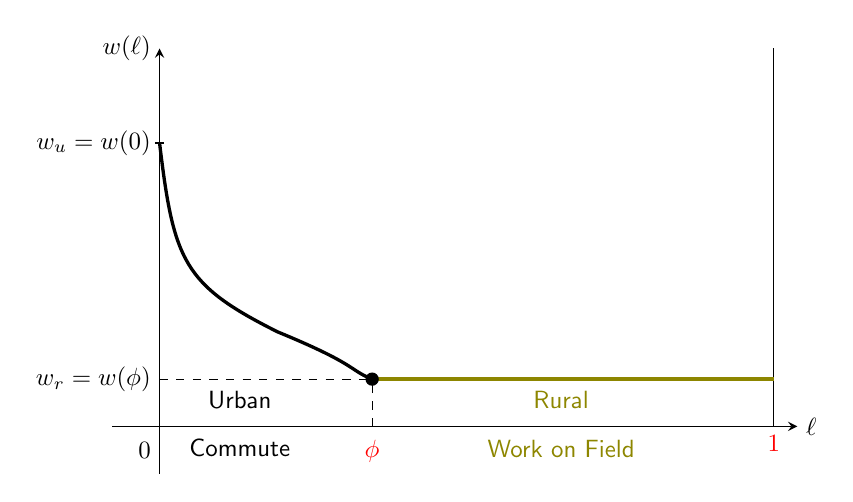
\begin{tikzpicture}[scale=0.6,every node/.style={scale=0.9}]



\pgfmathsetmacro{\WU}{6.0}
\pgfmathsetmacro{\WR}{1.0}
\pgfmathsetmacro{\PHI}{4.5}



  % xaxis
\draw[->,>=stealth,line width=0.5pt] (0,-1)--(0,8);
\draw (13.5,0) node (xaxis) [right] {$\ell$};
\draw[line width=0.5pt] (13,0)--(13,8);  % right y-axis
\draw (13,0) node [below] {\color{red}{$1$}};  % right y-axis label
\draw (0,-0.5) node (xaxis) [left] {$0$};
\draw[->,>=stealth,line width=0.5pt] (-1,0)--(13.5,0);%y axis


% axis labels

% \uncover<2->{

\draw (0,8) node[left] {$w(\ell)$};  % yaxis label
% intercept of w(0)
\draw[line width=0.5pt] (-0.1,\WU)--(0.1,\WU);
\draw (0,\WU) node (yaxis) [left] {$w_u=w(0)$};
% }

% \uncover<3->{
	% wage function
	\draw[line width=1.2pt, black] (0,\WU) ..controls +(0.3,-2.5) and +(-2,1).. (2.5,2) ..controls +(1.7,-0.7) and +(-0.5,0.2).. (\PHI,\WR);
% }


% \uncover<4->{
% wage from phi to 1
\draw[line width=1.3pt,olive](\PHI,\WR)--(13,\WR);

% dashed line for q(phi) and phi
\draw [dashed] (\PHI,0) |-(\PHI,\WR);
\draw [dashed] (0,\WR)--(\PHI,\WR);
\draw (0,\WR) node [left] {$w_r=w(\phi)$};
\fill (\PHI,\WR) circle[radius=4pt];
% \draw (5.3,4) node[right] {\color{red}{$\phi$}\textsf{: City fringe}};
\draw (\PHI,-0.1) node[below] {\color{red}{$\phi$}};

% text annotations
\draw (1.7,0.2) node[above] {\textsf{Urban}};
\draw (1.7,-0.08) node[below] {\textsf{Commute}};
\draw (8.5,0.2) node[above] {\textsf{\color{olive}{Rural}}};
\draw (8.5,-0.1) node[below] {\textsf{\color{olive}{Work on Field}}};
\end{tikzpicture}


% \end{document}